\documentclass[12pt]{article}
\usepackage{MinionPro}
\usepackage{CJK}
%\usepackage[scaled=0.85]{beramono}  %%% scaled=0.775
\usepackage[T1]{fontenc}
\usepackage{graphicx,booktabs,tabularx,psfrag}
\usepackage{xcolor}
\usepackage[a4paper]{geometry}
\usepackage{url}

\usepackage{pstool}



\usepackage{graphicx}
\begin{document}
\begin{CJK}{UTF8}{cwmb}
\renewcommand{\figurename}{圖}

\voffset=-1cm
\textwidth=5.6in
\textheight=9.2in

\newenvironment{num}
 {\leftmargini=6mm\leftmarginii=8mm
  \begin{enumerate}\itemsep=-2pt}
 {\end{enumerate}}

\newenvironment{sol}
 {\begin{quote}\mbox{}\llap{\color{blue}{解答:}\rule{10mm}{0pt}}\hspace*{-4pt}}{\end{quote}}


\thispagestyle{empty}
\fontsize{12}{20pt}\selectfont
\begin{center}
{\large\CJKfamily{cwyb}{經濟學原理下, 習題2}}\\[3mm]
劉彥佑 (R99628130)\\
李卿澄 (B97501046)\\
黃博億 (B99101014)\\
王祉婷 (B00704056)
\end{center}

\begin{num}
\item 
 \begin{num}
   \item 消費者物價指數圖形
\begin{figure}[htp]
\centering
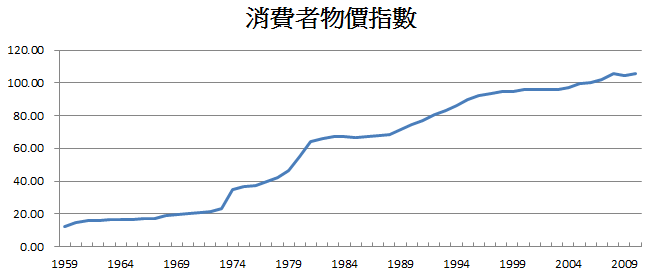
\includegraphics[scale=0.78]{CPI.png}
\caption{1951-2010之消費者物價指數,以2006年為基期}
\label{}
\end{figure}
   \item 平均的計算方式為將所有的物價膨脹率相加後除以物價膨脹率的個數。以1991-2000為例應有9個區間,9個物價膨脹率。
   \begin{itemize}
   \item 1991-2000之平均:2.4749\%
   \item 2001-2010之平均:1.0512\%
   \end{itemize}

 \end{num}

\item 650 ml「純喫茶」由去年一瓶20元到今年2月漲為一瓶25元。

\item 
  \begin{num}
   \item 若不論稅率某人所繳的稅皆相同,則其應稅所得乘上稅率為一定值。其應稅所得為該定值除以稅率:

$\frac{100\times0.5}{0.28} \approx 178.571$  (萬元) 

   \item 詳見圖2。
   \begin{figure}[htp]
\centering
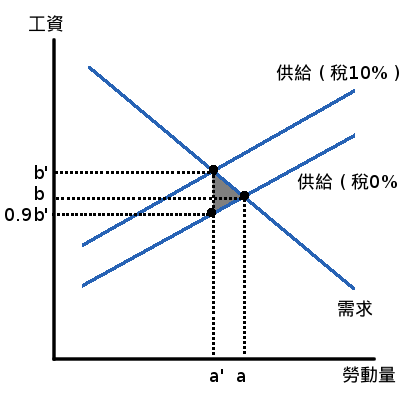
\includegraphics[scale=0.50]{dlot.png}
\caption{灰色三角形區域面積為課稅淨損失}
\label{}
\end{figure}
  \end{num}
\item 隨著人均GDP的成長,人們會意識到自身財產的增加,而更希望保護自身的財產不受他人侵害,對於財產權的保障需求自然提昇,隨著此需求的上升,財產權保障制度自然越趨完整。
\item 
	\begin{num}
		\item 勞動生產力參考課本公式為$\frac{1}{H\times\phi}\tilde{y}$,根據題設,H, $\phi$與$\tilde{y}$皆不改變,因此沒有勞動生產力之成長,故成長率為0。
		\item 平均每人生產毛額不變,只有每年增加1.4\%人口,由此可知隔年的國民生產毛額是其前一年的1.014倍,得國民生產毛額年成長率為1.4\%。
	\end{num}
\end{num}

\end{CJK}
\end{document}
